\documentclass[10pt, a4paper]{article}

\usepackage[paper=a4paper, left=1.5cm, right=1.5cm, bottom=1.5cm, top=1.5cm]{geometry}
\usepackage[utf8]{inputenc}
\usepackage[spanish]{babel}
\usepackage{graphicx}
\usepackage{multicol}
\usepackage[usenames,dvipsnames]{color}
\usepackage{amsmath}
\usepackage{verbatim}
\usepackage{footnote}
\usepackage{float}
\usepackage{amsfonts}
\usepackage{hyperref}
\usepackage{framed}
\usepackage{pdflscape}

\usepackage{pdfpages}

\usepackage{caratula}
\usepackage{userStories}

\materia{Ingeniería de Software II}

\titulo{Trabajo Práctico 1}
\subtitulo{Sprint Planning}

\integrante{Martín Alejandro Miguel}{181/09}{m2.march@gmail.com}
\integrante{Iván Postolski}{216/09}{ivan.postolski@gmail.com}
\integrante{Juan Manuel Martinez Caamaño}{276/09}{jmartinezcaamao@gmail.com}
\integrante{Matías Incem}{396/09}{matias.incem@gmail.com}
\integrante{Pablo Gauna}{334/09}{gaunapablo@gmail.com}


\begin{document}

\maketitle
\tableofcontents
\newpage

\section{Introducción}

El actual informe presenta el análisis, diseño y desarrollo inicial realizado para el producto \textbf{Precio Justo}. En el mismo se detallan el conjunto de \emph{user stories} que abarcan el desarrollo completo de la aplicación, incluyendo tanto las definiciones actuales como los puntos de extensión que se tendrán en cuenta. Se presenta además un primer \emph{diseño orientado a objetos} de la aplicación completa. Este tiene como objetivo ser expansible respecto de los distintos ejes de cambios considerados para esta instancia. Por último, se analiza el alcance, el proceso y el éxito de la primera iteración del proceso de desarrollo. 

\section{Análisis de la aplicación}

\subsection{Objetivo}

\textbf{Precio Justo} es una aplicación de recolección y procesamiento de datos masivos provistos por redes sociales. La intención es poder recopilar los precios más baratos para ciertos productos, de forma confiable y libre de intereses particulares. La elección del uso de las redes sociales para obtener los datos tiene como objetivo lograr imparcialidad en los mismos.

\subsection{Ejes de cambio}

Dentro de la resolución del objetivo de la aplicación se establecen, para una primera instancia, las siguientes restricciones, que pasan a conformar \emph{ejes de cambio} de la aplicación:

\paragraph{Obtención de datos}
\begin{itemize}
    \item \textbf{Origen de los datos:} En un primer lugar los datos a utilizar por la aplicación se obtendrán exclusivamente de \emph{twitter}. Dentro del flujo de datos del mismo, se espera filtrar aquellos que contengan información relevante para nuestros propósitos.
    \item \textbf{Formato de los tweets:} Considerando la restricción anterior, debe definirse bajo qué criterio un \emph{tweet} es útil. En una primera instancia los mismos deberán tener un formato similar a \textsf{$<$Producto$>$ $<$Precio$>$ $<$Unidad$>$ $<$Lugar$>$ \#PrecioJusto}, donde el \emph{hashtag} es indicador de que el \emph{tweet} está orientado a ser utilizado por nuestra aplicación. Se espera en un futuro poder precindir del \emph{hashtag} y poder interpretar formatos más flexibles.
    \item \textbf{Unidad de los productos:} Otra restricción impuesta para el procesamiento de datos es que los precios estén indicados en su valor por una cierta unidad, siendo restringida las unidades aceptadas para cada producto. Por ejemplo, para tomates se aceptan solo \emph{kilogramos}, y para leche el \emph{litro}.
    \item \textbf{Correctitud de los datos:} Una restricción implícita existente es que los mensajes a leer están bien escritos. Otra arista de cambio para la aplicación es poder soportar un cierto nivel de errores tipográficos en nuestra fuente cruda de datos.
\end{itemize}

\paragraph{Productos soportados}
Inicialmente la aplicación tendrá soporte para una cantidad limitada de productos, enfocándose principalmente en aquellos de primera necesidad. La misma debe ser suficientemente flexible para poder cambiar estos productos. 

\paragraph{Ubicación}
La aplicación debe informar el lugar donde puede comprarse el producto al precio establecido. Inicialmente esta información deberá estar presente en el mismo \emph{tweet} en formato de 'calle y altura'. Conciendo que \textbf{twitter} permite agregar como información del \emph{tweet} la posición geográfica del mismo, la misma podría utilizarse en reemplazo del texto explicitando la dirección. Se espera que la aplicación pueda usar estos datos. 

Por otra parte, es importante tener en cuenta que, de agregarse nuevas fuentes de datos a la aplicación, estas deben ser capaces de indicar dónde se consigue el producto al precio publicitado.

\paragraph{Resumen de la información}
Dentro de la definición de la aplicación se establece que debe permitírsele al usuario especificar como la información será tratada. En esto se definen las siguientes características.

\begin{itemize}
  \item \textbf{Resumen:} Dentro de la masividad de datos que tendremos para un producto, es necesario definir cómo estos se resumirán para el usuario. En primer lugar, se deben poder priorizar los precios más baratos. Además se definen otras estrategias para tratar los datos, como ser \emph{caminando lo menos posible}. El sistema debe permitir agregar nuevas estrategias fácilmente.
  \item \textbf{Filtrado:} Otra posibilidad de tratamiento de datos que se le ofrece al usuario es el filtrado de los mismos. En este momento se presentan dos filtros: por zona geográfica y por rango de precios. El sistema debe soportar agregar nuevos criterios fácilmente.
  \item \textbf{Productos:} En esta primera instancia de la aplicación se está poniendo como restricción que el usuario pueda elegir un solo producto para buscar. En la versión final, la aplicación debe permitirle hacer búsquedas de varios productos a la vez.
\end{itemize}

\paragraph{Veracidad de los datos} A pesar del supuesto donde los datos provistos por redes sociales son imparciales, esto no nos asegura que los datos sean siempre correctos. Es importante tener en cuenta que los precios suben o que algún precio reportado puede ser una oferta temporal. Para tratar con estas complejidades se decidió que el sistema podrá incorporar en un futuro una forma de especificar la vigencia del precio en caso de ser una oferta. En una primera instancia, la aplicación se compromente a utilizar solo datos que tengan una frescura suficiente de forma que puedan considerarse correctos.

Otra propuesta para esta temática es incrementar la interacción con el usuario y que este pueda votar o reportar las ofertas provistas según si fueron buenas o no. Este tipo de información nos permitiria eliminar datos falsos o desactualizados.

\paragraph{Presentación de los datos}
La visualización de ofertas que se le dará al usuario no se encuentra completamente definida en esta instancia, es por ello que el diseño del sistema debe ser capaz de adaptarse a distintas propuestas que puedan surgir en el mediano plazo. Una propuesta ya presente es que la aplicación incorpore la información de precios en un mapa.


\section{User Stories}

En esta sección presentamos las \textbf{user stories} definidas para el \emph{backlog} del proyecto. En las mismas se captura la extención completa de la aplicación. Durante el proceso de creación del \emph{product backlog} y la realización del \emph{sprint planning} se estudiaron distintas aristas del sistema a desarrollar y el problema a resolver. Las historias planteadas reflejan distintas resoluciones tomadas respecto al alcance de la aplicación. Así mismo en las \emph{stories} se declararon cuestiones que no podían ser resueltas en esta primera etapa. Este es el caso de los \textbf{epics}. 

Son sumamente generales y deberán ser desarrolladas en el futuro. Cada uno representa uno de los nortes planteados por los \textsf{product owners}. Alguno de los \textbf{epics} se solapan con otras historias planteadas, lo cual significa que el mismo está siendo abordado. En este caso el \textbf{epic} toma relevancia para recordar cual es el objetivo global que se busca y generar planteos respecto a correcciones y nuevas funcionalidades que pueda darse al producto final. 

\subsection{Sprint Backlog}
\userStory	{US145} % ID en el Rally
	{Realizar un primer análisis y diseño de la aplicación} % titulo
	{En una primera instancia es importante comprender la naturaleza de la\\
aplicación, entender los requerimientos, sugerir propuestas para resolverlos y\\
bocetar una estructura global que permita la división del trabajo entre los\\
integrantes del grupo.\\
  \\
También es necesario definir un camino de desarrollo, priorizar los\\
requerimientos y establecer líneas de expansión de la aplicación que sean\\
deseables.\\
  \\
\textbf{Criterios de aceptación:}\\
* El grupo de trabajo acordará en un lenguaje/código común para realizar el diseño orientado a objetos.  \\
* El grupo poseerá un boceto básico del diseño global de la aplicación.  \\
* Los integrantes podrán comenzar a trabajar por separado con un conocimiento básico de las actividades que el grupo debe realizar.  \\
} % descripcion
	{} % criterios de aceptacion
	{8.0} % story points
	{Martin M} % story owner
	{Primera} % iteracion (Primera o ``no definida'')
	{Accepted} % estado (completada, bloqueada, etc.)


\vspace{20pt}

\userStory	{US144} % ID en el Rally
	{Como desarrollador quiero buscar un mecanismo que permita estandarizar los archivos de código Python} % titulo
	{Python es sensible a la identación, y en el trabajo en equipo puede ser\\
problemático que los integrantes acostumbren usar distintos criterios de\\
tabulación.\\
  \\
Es necesario encontrar algún mecanismo/programa/utilitario que ayude a manejar\\
este y otros problemas de formato de código.\\
  \\
\textbf{Criterios de aceptación:}\\
* Los integrantes del grupo trabajarán con código Python estandarizado  \\
} % descripcion
	{} % criterios de aceptacion
	{2.0} % story points
	{Martin M} % story owner
	{Primera} % iteracion (Primera o ``no definida'')
	{Accepted} % estado (completada, bloqueada, etc.)


\vspace{20pt}

\userStory	{US143} % ID en el Rally
	{Como desarrollador quiero tener un mecanismo para hacer tests unitarios} % titulo
	{Se quiere disponer de un software que nos permita realizar tests unitarios. El\\
mecanismo debe haber sido testeado en su facilidad de uso y extensibilidad\\
creando tests.\\
  \\
  \\
\textbf{Criterios de aceptación:}\\
  \\
* Se dispondrá de un mecanismo de fácil extensión para poder testear funcionalidades unitarias. \\
} % descripcion
	{} % criterios de aceptacion
	{3.0} % story points
	{Martin M} % story owner
	{Primera} % iteracion (Primera o ``no definida'')
	{Accepted} % estado (completada, bloqueada, etc.)

	\task	{TA192} % ID en el Rally
		{Investigar bibliotecas o mecanismos para hacer unit testing en el lenguaje de programación del servidor} % titulo
		{El código del servidor está escrito en Python, por lo que se investigará el\\
funcionamiento de PyUnit para realizar tests unitarios.\\
} % descripcion
		{3.0} % horas estimadas
		{Juan M} % story owner
		{0.0} % horas faltantes
		{Completed} % estado (completada, bloqueada, etc.)

	\task	{TA193} % ID en el Rally
		{Implementar tests de ejemplo con el mecanismo elegido que sirvan de modelo para futuros tests} % titulo
		{\\
} % descripcion
		{1.0} % horas estimadas
		{Martin M} % story owner
		{1.0} % horas faltantes
		{Defined} % estado (completada, bloqueada, etc.)


\vspace{20pt}

\userStory	{US101} % ID en el Rally
	{Como desarrollador quiero investigar las opciones disponibles para obtener información de Twitter} % titulo
	{Queremos conocer y contrastar las alternativas sobre la obtención y\\
almacenamiento de la información obtenida desde Twitter.\\
  \\
En principio tenemos las siguientes funcionalidades, en las que tenemos que\\
decidir entre dos implementaciones en cada una:\\
* Almacenar la información vs. obtenerla en cada búsqueda del usuario.\\
* Investigar la Search REST API vs. Streaming API de Twitter.\\
  \\
\textbf{Criterios de aceptación:}\\
* El grupo de trabajo conocerá el método para obtener la información desde Twitter  \\
} % descripcion
	{} % criterios de aceptacion
	{5.0} % story points
	{Martin M} % story owner
	{Primera} % iteracion (Primera o ``no definida'')
	{Accepted} % estado (completada, bloqueada, etc.)

	\task	{TA35} % ID en el Rally
		{Investigar cómo funcionan las APIs (REST y Streaming), junto con las SDK de Twitter} % titulo
		{\\
} % descripcion
		{4.0} % horas estimadas
		{Ivan P} % story owner
		{0.0} % horas faltantes
		{Completed} % estado (completada, bloqueada, etc.)

	\task	{TA36} % ID en el Rally
		{Discutir ventajas y desventajas de cada API y elegir una} % titulo
		{\\
} % descripcion
		{2.0} % horas estimadas
		{} % story owner
		{0.0} % horas faltantes
		{Completed} % estado (completada, bloqueada, etc.)

	\task	{TA37} % ID en el Rally
		{Investigar y elegir cómo y cuándo vamos a conseguir los datos} % titulo
		{Se desea tener un método para conseguir datos para responder una consulta.\\
Podemos obtenerlos siempre desde Twitter y no guardar nada, o bien podemos\\
almacenarlos de antemano y usarlos cuando debemos responder una consulta.\\
Revisar como impacta en el sprint backlog esta decisión.\\
} % descripcion
		{4.0} % horas estimadas
		{} % story owner
		{0.0} % horas faltantes
		{Completed} % estado (completada, bloqueada, etc.)


\vspace{20pt}

\userStory	{US99} % ID en el Rally
	{Como PO espero que la información sea obtenida a través de Twitter} % titulo
	{El Product Owner desea que el sistema pueda comunicarse con Twitter para\\
recibir información. Por lo tanto, es necesario asegurarse de que podemos\\
recibir datos usando una conexión con Twitter, y que podemos decodificar y\\
entender los datos recibidos.\\
  \\
\textbf{Criterios de aceptación:}\\
* El sistema tendrá una conexión con la API de Twitter y podrá descargar los datos que necesita  \\
* Toda la información obtenida podrá ser leída por el sistema, los datos útiles deberán ser identificados, separados y convertidos a un formato utilizable por la aplicación. \\
  \\
Business value: 8\\
} % descripcion
	{} % criterios de aceptacion
	{5.0} % story points
	{Ivan P} % story owner
	{Primera} % iteracion (Primera o ``no definida'')
	{Accepted} % estado (completada, bloqueada, etc.)

	\task	{TA40} % ID en el Rally
		{Implementar el conector para Twitter} % titulo
		{Necesitamos un conector que pueda realizar una llamada al servidor de Twitter\\
y descargar datos.\\
* El conector debe poder conectarse a Twitter autenticándose con OAuth2\\
* El conector debe poder obtener los mensajes de Twitter con un hashtag particular, en nuestro caso, \#precioJusto\\
} % descripcion
		{6.0} % horas estimadas
		{} % story owner
		{0.0} % horas faltantes
		{Completed} % estado (completada, bloqueada, etc.)

	\task	{TA41} % ID en el Rally
		{Registrar la aplicación en Twitter} % titulo
		{Es necesario dar de alta la aplicación en Twitter, para obtener las\\
credenciales para usar la API. Esto es requerido para cualquier aplicación que\\
quiera trabajar con Twitter.\\
} % descripcion
		{2.0} % horas estimadas
		{} % story owner
		{0.0} % horas faltantes
		{Completed} % estado (completada, bloqueada, etc.)

	\task	{TA42} % ID en el Rally
		{Traducir los datos obtenidos de Twitter al modelo interno de representación} % titulo
		{Debemos tener un traductor que lea los datos que conforman un tweet y los\\
convierta en objetos de nuestro modelo, fundamentalmente en un objeto\\
"oferta".\\
} % descripcion
		{4.0} % horas estimadas
		{} % story owner
		{0.0} % horas faltantes
		{Completed} % estado (completada, bloqueada, etc.)


\vspace{20pt}

\userStory	{US113} % ID en el Rally
	{Como desarrollador quiero reconocer tweets útiles y convertirlos a ofertas} % titulo
	{Cuando el sistema recibe datos de Twitter, necesita poder identificar aquellos\\
que tienen información útil. Esto se determina de acuerdo a su formato. En\\
esta etapa del proyecto, los tweets que son útiles son aquellos que cumplen el\\
formato "$<$ Producto$>$  $<$ Precio$>$  $<$ Unidad$>$  $<$ Lugar$>$  \#precioJusto", y además, tengan\\
un producto válido, una unidad soportada por el producto, y un precio y lugar\\
válidos. Es necesario identificar los tweets válidos y extraer la información\\
contenida en ellos.\\
  \\
\textbf{Criterios de aceptación:}\\
* La aplicación conocerá los productos y unidades aceptados por los administradores y podrá contrastarlos con los datos de los tweets.  \\
* Si un tweet con el hashtag \#precioJusto no tiene información correcta o no es relevante, deberá ser ignorado por el sistema.  \\
* Si un tweet con el hashtag es relevante y válido, el sistema deberá componer un objeto 'oferta' que contenga la información dada por dicho tweet.\\
} % descripcion
	{} % criterios de aceptacion
	{5.0} % story points
	{Martin M} % story owner
	{Primera} % iteracion (Primera o ``no definida'')
	{Accepted} % estado (completada, bloqueada, etc.)

	\task	{TA135} % ID en el Rally
		{Implementar un mecanismo para obtener la lista de productos y sus unidades} % titulo
		{Para poder validar los tweets, es necesario conocer la lista de productos\\
válidos y de unidades válidas para cada producto. El sistema puede pedir esta\\
lista.\\
} % descripcion
		{3.0} % horas estimadas
		{} % story owner
		{0.0} % horas faltantes
		{Completed} % estado (completada, bloqueada, etc.)

	\task	{TA139} % ID en el Rally
		{Implementar el parser que reconozca si el formato de un tweet es correcto} % titulo
		{Se deberá reconocer si el tweet tiene la información necesaria de producto,\\
precio, unidad y lugar.\\
El formato básico a soportar es: $<$ Producto$>$  $<$ Precio$>$  $<$ Unidad$>$  $<$ Lugar$>$ \\
\#PrecioJusto\\
} % descripcion
		{5.0} % horas estimadas
		{} % story owner
		{0.0} % horas faltantes
		{Completed} % estado (completada, bloqueada, etc.)

	\task	{TA140} % ID en el Rally
		{Con los tweets útiles reconocidos, extraer la información para generar una oferta} % titulo
		{Se deben separar los datos validados del tweet para construir un objeto\\
Oferta, que posea la información necesaria y pueda ser leído por la\\
aplicación.\\
} % descripcion
		{2.0} % horas estimadas
		{} % story owner
		{0.0} % horas faltantes
		{Completed} % estado (completada, bloqueada, etc.)


\vspace{20pt}

\userStory	{US106} % ID en el Rally
	{Como desarrollador quiero tener una base para la API REST del backend} % titulo
	{Se espera implementar un código inicial del backend que permita agregar\\
fácilmente nuevos métodos a la interfaz REST, los cuales permitirán acceder al\\
funcionamiento interno del mismo.\\
  \\
\textbf{Criterios de aceptación:}\\
* El backend dispondrá de un método /status que permita verificar si está funcionando correctamente.   \\
* El código de este método será fácilmente replicable para agregar nuevas funcionalidades.\\
} % descripcion
	{} % criterios de aceptacion
	{5.0} % story points
	{Martin M} % story owner
	{Primera} % iteracion (Primera o ``no definida'')
	{Accepted} % estado (completada, bloqueada, etc.)

	\task	{TA111} % ID en el Rally
		{Implementar una operación básica de busqueda de ofertas en nuestro servicio} % titulo
		{Esta task cubre la implementacion base del servicio.\\
} % descripcion
		{4.0} % horas estimadas
		{Martin M} % story owner
		{0.0} % horas faltantes
		{Completed} % estado (completada, bloqueada, etc.)

	\task	{TA141} % ID en el Rally
		{Investigar bibliotecas para la implementación del servicio} % titulo
		{Investigar distintas bibliotecas útiles para la implementación del servicio.\\
Como primera instancia se presenta la siguiente:\\
  \\
[http://www.cherrypy.org/](http://www.cherrypy.org/)\\
} % descripcion
		{4.0} % horas estimadas
		{Martin M} % story owner
		{0.0} % horas faltantes
		{Completed} % estado (completada, bloqueada, etc.)


\vspace{20pt}

\userStory	{US124} % ID en el Rally
	{Como desarrollador quiero implementar la base del mecanismo de estrategias y filtros} % titulo
	{Se desea implementar el código básico que se aprovechará en las futuras\\
implementaciones de filtros y estrategias.\\
En este código debe tomarse el total de ofertas y devolver un subconjunto,\\
definido por los filtros y  las estrategias configuradas.\\
Un filtro toma un conjunto de ofertas y devuelve el subconjunto de ellas que\\
cumple un criterio determinado, por ejemplo, su precio es menor a 5 pesos, o\\
su dirección está en determinada calle. Otra forma de entender este concepto\\
es como una función Oferta -$>$  Bool que responde si la oferta cumple el\\
criterio o no.\\
Una estrategia toma un conjunto de ofertas y las ordena de acuerdo a una\\
cualidad, por ejemplo, de menor a mayor precio. Notar que en algunos casos, el\\
resultado final no aprovechará la lista ordenada completa (por ejemplo, podría\\
necesitar solo el primer elemento), por lo que no siempre se necesita hacer\\
todo el procedimiento.\\
  \\
\textbf{Criterios de aceptación:}\\
* El sistema tendrá código que le permita llamar a un manejador de filtros y estrategias.  \\
* Se podrá invocar la aplicación de un filtro o estrategia "nulo". Esta operación no tendrá ningún efecto en los datos, pero su código será fácilmente extensible para agregar funcionalidades.  \\
  \\
} % descripcion
	{} % criterios de aceptacion
	{5.0} % story points
	{Juan M} % story owner
	{Primera} % iteracion (Primera o ``no definida'')
	{Accepted} % estado (completada, bloqueada, etc.)

	\task	{TA143} % ID en el Rally
		{Testear la implementación mediante un filtro y una estrategia de prueba} % titulo
		{\\
} % descripcion
		{3.0} % horas estimadas
		{Juan M} % story owner
		{0.0} % horas faltantes
		{Completed} % estado (completada, bloqueada, etc.)


\vspace{20pt}

\userStory	{US147} % ID en el Rally
	{Como usuario del backend quiero conocer las estrategias provistas por el sistema} % titulo
	{En las capas de frontend que le presenten funcionalidad al usuario deseo poder\\
mostrarle qué estrategias tiene disponible para resumir la información\\
provista por el sistema.\\
  \\
\textbf{Criterios de aceptación:}\\
* La interfaz rest debe exponer la lista de estrategias disponibles mediante un método /strategies\\
  \\
\textbf{Bussiness Value:} 5\\
} % descripcion
	{} % criterios de aceptacion
	{3.0} % story points
	{Matias I} % story owner
	{Primera} % iteracion (Primera o ``no definida'')
	{Accepted} % estado (completada, bloqueada, etc.)


\vspace{20pt}

\userStory	{US104} % ID en el Rally
	{Como desarrollador quiero filtrar las ofertas según un rango de precios} % titulo
	{Se debe lograr un código que adquiera los datos de las ofertas y los filtre\\
según un rango de precios determinado. Las ofertas que estén fuera del rango\\
deberán ser descartadas. Esta funcionalidad complementa la desarrollada en la\\
US96, que permite que el sistema obtenga un rango de precios entre los datos\\
enviados por el usuario.\\
  \\
\textbf{Criterios de aceptación:}\\
* Tenemos ofertas con precios que van desde X hasta Y, y elegimos filtrar desde A hasta Z.   \\
* Luego de aplicado el filtro, las ofertas resultantes serán todas las que cumplan con los otros criterios de la consulta y tengan precio mayor o igual a A y menor o igual a Z.  \\
} % descripcion
	{} % criterios de aceptacion
	{2.0} % story points
	{Ivan P} % story owner
	{Primera} % iteracion (Primera o ``no definida'')
	{Accepted} % estado (completada, bloqueada, etc.)

	\task	{TA56} % ID en el Rally
		{Implementar el filtrado de las ofertas por rango de precios} % titulo
		{El código debe acoplarse al mecanismo de filtros y estrategias implementado en\\
la US124\\
} % descripcion
		{4.0} % horas estimadas
		{Ivan P} % story owner
		{0.0} % horas faltantes
		{Completed} % estado (completada, bloqueada, etc.)


\vspace{20pt}

\userStory	{US96} % ID en el Rally
	{Como usuario espero realizar búsquedas filtrando por un rango de precios} % titulo
	{Cuando el usuario realiza una consulta, puede querer definir un rango de\\
precios, de forma que en la respuesta del sistema solo aparezcan las ofertas\\
cuyos precios son mayores a un valor mínimo y menores a un valor máximo.\\
Nota: Esta story describe las atribuciones del frontend. La funcionalidad que\\
permite que el backend realice un filtro sobre sus datos se encuentra en la\\
US104.\\
  \\
\textbf{Criterios de aceptación:}\\
  \\
* La inferfaz permitirá ingresar, de forma opcional, un rango de precios, formado por un valor MIN y un valor MAX.  \\
* Si los parámetros son ingresados incorrectamente la interfaz debe decirlo. Esto puede ocurrir si el rango es inválido o los números están mal escritos.\\
* Todas las ofertas sugeridas al finalizar la consulta se encontrarán dentro del rango explicitado.  \\
  \\
\textbf{Bussiness Value:} 5\\
} % descripcion
	{} % criterios de aceptacion
	{5.0} % story points
	{Juan M} % story owner
	{Primera} % iteracion (Primera o ``no definida'')
	{Accepted} % estado (completada, bloqueada, etc.)

	\task	{TA59} % ID en el Rally
		{Implementar en el cliente un medio para establecer el tipo de consulta "por rango" y el rango establecido} % titulo
		{La interfaz de usuario necesita tener una funcionalidad para elegir si se\\
incluye un rango de precios en la búsqueda. Además, en caso de que se lo\\
elija, también debe tener un campo donde ingresar precio máximo y mínimo.\\
} % descripcion
		{4.0} % horas estimadas
		{Juan M} % story owner
		{0.0} % horas faltantes
		{Completed} % estado (completada, bloqueada, etc.)

	\task	{TA60} % ID en el Rally
		{Implementar la comunicación del cliente con el backend, enviando los parámetros} % titulo
		{El backend debe tener un método REST para recibir la consulta. El cliente debe\\
utilizar este método de forma correcta enviando los parámetros.\\
} % descripcion
		{2.0} % horas estimadas
		{Juan M} % story owner
		{0.0} % horas faltantes
		{Completed} % estado (completada, bloqueada, etc.)

	\task	{TA61} % ID en el Rally
		{Implementar la recepción y exhibición de los datos de respuesta en el frontend} % titulo
		{El cliente debe poder recibir la respuesta del backend y exponerla al usuario\\
a través de su interfaz.\\
} % descripcion
		{3.0} % horas estimadas
		{Juan M} % story owner
		{0.0} % horas faltantes
		{Completed} % estado (completada, bloqueada, etc.)


\vspace{20pt}

\subsection{Product Backlog}
\userStory	{US110} % ID en el Rally
	{Como desarrollador quiero investigar cómo determinar zonas geográficas} % titulo
	{Es necesario establecer un criterio para delimitar las zonas que servirán de\\
filtro en nuestra aplicación.\\
Algunas opciones son:\\
  \\
* Utilizar la API de google maps si es que tiene en ella información de zonas\\
* Si existe, utilizar la API del mapa del Gobierno de la Ciudad para usar las zonas delimitadas en la misma\\
* Definir las zonas manualmente en nuestra aplicación\\
  \\
También se debe determinar si es necesario recortar inicialmente el alcance\\
total de la aplicación a, por ejemplo, Capital Federal.\\
  \\
\textbf{Criterios de aceptación:}\\
* El grupo de trabajo conocerá el concepto de zona que se utilizará, así como la manera de operar con las zonas.  \\
} % descripcion
	{} % criterios de aceptacion
	{5.0} % story points
	{Martin M} % story owner
	{no definida} % iteracion (Primera o ``no definida'')
	{Defined} % estado (completada, bloqueada, etc.)


\vspace{20pt}

\userStory	{US88} % ID en el Rally
	{Epic: Como usuario quiero obtener la direccion, precio y unidad del producto respetando los filtros ingresados} % titulo
	{\\
} % descripcion
	{} % criterios de aceptacion
	{30.0} % story points
	{Martin M} % story owner
	{no definida} % iteracion (Primera o ``no definida'')
	{In-Progress} % estado (completada, bloqueada, etc.)


\vspace{20pt}

\userStory	{US82} % ID en el Rally
	{Como usuario espero realizar búsquedas filtrando por zona} % titulo
	{El sistema debe permitir una funcionalidad en la que el usuario pueda elegir e\\
indicar una zona al momento de hacer su consulta, en caso de que lo desee; si\\
lo hace, las respuestas que reciba deberán estar restringidas a ofertas dentro\\
de dicha zona.\\
  \\
Queda pendiente definir el concepto de zona, y decidir si estarán fijadas por\\
el sistema o pueden ser delimitadas por el usuario durante la consulta.\\
  \\
Esta historia es dependente de la investigación previa realizada en la US110\\
  \\
\textbf{Criterios de aceptación:}\\
* El usuario podrá elegir buscar ofertas por zona, y en dicho caso, podrá especificar una zona.  \\
* Todas las direcciones de las ofertas devueltas en el resultado estarán dentro de la zona elegida por el usuario.\\
  \\
\textbf{Bussiness Value:} 6\\
} % descripcion
	{} % criterios de aceptacion
	{8.0} % story points
	{Martin M} % story owner
	{no definida} % iteracion (Primera o ``no definida'')
	{Defined} % estado (completada, bloqueada, etc.)

	\task	{TA46} % ID en el Rally
		{Implementar el filtro por zonas.} % titulo
		{\\
} % descripcion
		{10.0} % horas estimadas
		{} % story owner
		{10.0} % horas faltantes
		{Defined} % estado (completada, bloqueada, etc.)


\vspace{20pt}

\userStory	{US83} % ID en el Rally
	{Como usuario quiero realizar búsquedas con la estrategia "gastando lo menos posible"} % titulo
	{Cuando se realiza una consulta, se puede elegir la estrategia "gastando lo\\
menos posible", que consiste en seleccionar las ofertas de precio mínimo entre\\
todas las ofertas válidas, y solamente mostrar esas en el resultado.\\
  \\
\textbf{Criterios de aceptación:}\\
* Cuando el usuario haga una consulta, podrá elegir que se aplique la estrategia "gastando lo menos posible"  \\
* Si está seleccionada, el sistema solamente retornará como respuesta las ofertas con el precio más económico entre las que encontró para un determinado producto. \\
  \\
\textbf{Bussiness Value:} 9\\
} % descripcion
	{} % criterios de aceptacion
	{3.0} % story points
	{Martin M} % story owner
	{no definida} % iteracion (Primera o ``no definida'')
	{Defined} % estado (completada, bloqueada, etc.)


\vspace{20pt}

\userStory	{US85} % ID en el Rally
	{Como usuario quiero elegir un producto entre los soportados por el sistema para obtener precios de dicho producto} % titulo
	{Se desea tener una funcionalidad básica del sistema, que es la siguiente: el\\
usuario ingresa el nombre de un producto válido, y el sistema devuelve un\\
conjunto de ofertas relacionadas con dicho producto, las cuales se consiguen a\\
partir de información de tweets.\\
  \\
\textbf{Criterios de aceptación:}\\
* El usuario podrá elegir un producto para realizar su consulta, y sabrá si el producto elegido es válido.  \\
* El sistema devolverá una lista de ofertas para el producto, que incluyen información de precio por unidad y lugar. \\
  \\
\textbf{Bussiness Value:} 3\\
} % descripcion
	{} % criterios de aceptacion
	{3.0} % story points
	{Matias I} % story owner
	{Primera} % iteracion (Primera o ``no definida'')
	{Accepted} % estado (completada, bloqueada, etc.)

	\task	{TA108} % ID en el Rally
		{Implementar una forma de exportar los productos soportados en el backend} % titulo
		{La interfaz REST debe exportar, mediante un método /products, la lista de\\
productos soportados junto con su unidad.\\
} % descripcion
		{4.0} % horas estimadas
		{Juan M} % story owner
		{0.0} % horas faltantes
		{Completed} % estado (completada, bloqueada, etc.)

	\task	{TA109} % ID en el Rally
		{Implementar la obtención de los productos en el frontend} % titulo
		{Se necesita que el cliente de la aplicación consulte satisfactoriamente al\\
backend y pueda obtener la lista de los productos soportados y sus unidades\\
para operar con ellos o presentárselos al usuario.\\
} % descripcion
		{4.0} % horas estimadas
		{Juan M} % story owner
		{0.0} % horas faltantes
		{Completed} % estado (completada, bloqueada, etc.)

	\task	{TA110} % ID en el Rally
		{Mostrar al usuario la lista de productos soportados y permitirle elegir un producto} % titulo
		{La interfaz con la que se comunica el usuario le debe dar a elegir al mismo\\
uno o más productos de la lista de productos válidos, y esta selección debe\\
estar visible durante el resto de la consulta.\\
} % descripcion
		{4.0} % horas estimadas
		{Juan M} % story owner
		{0.0} % horas faltantes
		{Completed} % estado (completada, bloqueada, etc.)


\vspace{20pt}

\userStory	{US105} % ID en el Rally
	{Como desarrollador quiero tener una implementación básica del frontend y backend} % titulo
	{Se necesita tener un código del backend que provea una API para comunicarse\\
con el frontend. También necesitamos definir un frontend que sepa comunicarse\\
con esa API y además provea un interfaz para que el usuario pueda realizar\\
consultas.\\
  \\
\textbf{Criterios de aceptación:}\\
* El backend deberá ponerse en funcionamiento y proveer una API REST.  \\
* El frontend tendrá una interfaz visible para el usuario. Además podrá comunicarse con la API del backend.  \\
* El código podrá ser fácilmente extensible para agregar funcionalidad.\\
} % descripcion
	{} % criterios de aceptacion
	{13.0} % story points
	{Juan M} % story owner
	{Primera} % iteracion (Primera o ``no definida'')
	{Accepted} % estado (completada, bloqueada, etc.)

	\task	{TA145} % ID en el Rally
		{Instalar todos los componentes necesarios para el desarrollo} % titulo
		{Necesitamos que todos los integrantes del grupo instalemos las aplicaciones\\
que se necesitan para desarrollar el software: Python, Tweepy, Git.\\
} % descripcion
		{5.0} % horas estimadas
		{Juan M} % story owner
		{0.0} % horas faltantes
		{Completed} % estado (completada, bloqueada, etc.)

	\task	{TA146} % ID en el Rally
		{Crear el proyecto inicial} % titulo
		{Se debe crear un proyecto que incluya espacio para el código fuente, la\\
documentación y los diagramas de diseño. Cada uno de ellos deberá ser\\
completado a medida que avanza el proyecto.\\
} % descripcion
		{4.0} % horas estimadas
		{Juan M} % story owner
		{0.0} % horas faltantes
		{Completed} % estado (completada, bloqueada, etc.)

	\task	{TA147} % ID en el Rally
		{Agregar un primer código que le dé cierta funcionalidad al cliente frontend} % titulo
		{Se necesita un código básico de un frontend que pueda comunicarse con el\\
backend de nuestro sistema a través de una API, y con el usuario por medio de\\
una interfaz.\\
} % descripcion
		{4.0} % horas estimadas
		{Juan M} % story owner
		{0.0} % horas faltantes
		{Completed} % estado (completada, bloqueada, etc.)

	\task	{TA148} % ID en el Rally
		{Generar el código de la interfaz que siente las bases para la fácil implementación de agregados} % titulo
		{Se debe hacer un primer esbozo de una interfaz de usuario.\\
} % descripcion
		{5.0} % horas estimadas
		{Juan M} % story owner
		{0.0} % horas faltantes
		{Completed} % estado (completada, bloqueada, etc.)

	\task	{TA149} % ID en el Rally
		{Implementar la conexión con el servicio REST} % titulo
		{El frontend debe ser capaz de comunicarse con el backend, por medio de la API\\
REST de este último.\\
} % descripcion
		{4.0} % horas estimadas
		{Juan M} % story owner
		{0.0} % horas faltantes
		{Completed} % estado (completada, bloqueada, etc.)

	\task	{TA150} % ID en el Rally
		{Validar los funcionamientos generados} % titulo
		{Es necesario testear la funcionalidad del frontend y backend en cuanto a\\
comunicación.\\
} % descripcion
		{4.0} % horas estimadas
		{Juan M} % story owner
		{0.0} % horas faltantes
		{Completed} % estado (completada, bloqueada, etc.)


\vspace{20pt}

\userStory	{US102} % ID en el Rally
	{Como usuario quiero realizar búsquedas filtrando por la estrategia 'caminando lo menos posible'} % titulo
	{En una consulta del usuario se puede elegir la estrategia 'caminando lo menos\\
posible', que elige, entre las ofertas válidas para un producto, aquella que\\
se encuentra más cerca de la posición actual del usuario.\\
Considerar: la funcionalidad será distinta si se permite la búsqueda\\
simultánea de varios productos (Ver US126).\\
  \\
\textbf{Criterios de aceptación:}\\
* En la interfaz deberá figurar la opción para elegir la estrategia 'caminando lo menos posible'\\
* El resultado de aplicar esta estrategia deberá mostrar la oferta que cumpla con los demás filtros (rango, zona, etc.), y además sea la mas cercana a la posición del usuario.\\
* En caso de que el sistema no logre ubicar al usuario, un error será mostrado al usuario, indicando que no es posible ejecutar la consulta porque el sistema no conoce su ubicación.\\
  \\
\textbf{Bussiness Value:} 8\\
} % descripcion
	{} % criterios de aceptacion
	{3.0} % story points
	{Martin M} % story owner
	{no definida} % iteracion (Primera o ``no definida'')
	{Defined} % estado (completada, bloqueada, etc.)


\vspace{20pt}

\userStory	{US100} % ID en el Rally
	{Como PO quiero enfocarme en productos de primera necesidad.} % titulo
	{Desde los requerimientos iniciales se estableció que el sistema se enfocará en\\
buscar ofertas para productos de primera necesidad. Cuales son estos productos\\
deberá ser definido por el product owner.\\
  \\
\textbf{Criterios de aceptación:}\\
* El sistema admite como productos a buscar aquellos definidos por el product owner.\\
} % descripcion
	{} % criterios de aceptacion
	{1.0} % story points
	{Martin M} % story owner
	{no definida} % iteracion (Primera o ``no definida'')
	{Defined} % estado (completada, bloqueada, etc.)

	\task	{TA54} % ID en el Rally
		{Consultar al PO qué productos con qué unidades son de interés} % titulo
		{\\
} % descripcion
		{1.0} % horas estimadas
		{} % story owner
		{1.0} % horas faltantes
		{Defined} % estado (completada, bloqueada, etc.)

	\task	{TA55} % ID en el Rally
		{Modificar el sistema para que tenga en cuenta las especificaciones del PO} % titulo
		{\\
} % descripcion
		{1.0} % horas estimadas
		{} % story owner
		{1.0} % horas faltantes
		{Defined} % estado (completada, bloqueada, etc.)


\vspace{20pt}

\userStory	{US89} % ID en el Rally
	{Como PO espero poder agregar y eliminar productos de la lista de productos soportados junto con su respectiva unidad} % titulo
	{El sistema está pensado para tratar con productos "de primera necesidad", y el\\
objetivo es tener una lista cerrada de productos soportados. En principio esta\\
lista es fija, pero se quiere que en un futuro pueda ser modificada, agregando\\
o quitando productos según las decisiones del Product Owner, que puede querer\\
que un producto sea o no soportado por la aplicación.\\
  \\
\textbf{Criterios de aceptación:}\\
* Un administrador del sistema podrá incluir un nuevo producto para ser soportado por la aplicación, junto con una o más unidades de medida asociadas. Los usuarios podrán consultar por dicho producto luego de que haya sido dado de alta, y el funcionamiento deberá ser correcto al igual que con los productos originales.  \\
* Un administrador podrá eliminar un producto de la lista. Los usuarios no podrán volver a consultar sobre dicho producto en la aplicación.  \\
* Un administrador podrá agregar una nueva unidad asociada a un producto existente. Las respuestas a las consultas de dicho producto incluirán ofertas con dicho producto y unidad. También podrá ser eliminada una unidad existente, y las ofertas que usen esa unidad no aparecerán.\\
} % descripcion
	{} % criterios de aceptacion
	{8.0} % story points
	{Martin M} % story owner
	{no definida} % iteracion (Primera o ``no definida'')
	{Defined} % estado (completada, bloqueada, etc.)


\vspace{20pt}

\userStory	{US87} % ID en el Rally
	{Como usuario quiero que la información consultada se muestre en un mapa, indicando los lugares de compra y los precios de los productos} % titulo
	{El mapa es un método visualmente eficiente para mostrar las ofertas que son\\
respuesta a una consulta del usuario. La dirección puede ser señalada con un\\
punto en el mapa, y el resto de la información puede verse en el epígrafe que\\
acompaña al punto.\\
  \\
\textbf{Criterios de aceptación:}\\
* Cuando el usuario realiza una consulta, podrá elegir que los resultados se muestren en un mapa.  \\
* Las direcciones de todas las ofertas resultantes aparecerán como puntos en el mapa, y los datos restantes de las ofertas estarán escritos al costado de cada punto. \\
  \\
\textbf{Bussiness Value:} 7\\
} % descripcion
	{} % criterios de aceptacion
	{13.0} % story points
	{Martin M} % story owner
	{no definida} % iteracion (Primera o ``no definida'')
	{Defined} % estado (completada, bloqueada, etc.)

	\task	{TA105} % ID en el Rally
		{Investigar la API de google maps} % titulo
		{En la api de google maps es necesario investigar cómo:\\
  \\
* Ingresarle los datos de los lugares a mostrar\\
* Ingresar junto con los puntos de interés datos de los mismos\\
* Mostrar el mapa en el cliente\\
} % descripcion
		{} % horas estimadas
		{} % story owner
		{} % horas faltantes
		{Defined} % estado (completada, bloqueada, etc.)

	\task	{TA106} % ID en el Rally
		{Implementar en el cliente la comunicación con Google Maps} % titulo
		{El código implementado debe tomar los resultados devueltos por el backend y\\
traducirlos y enviárselos a la api de google maps para que cree el mapa con\\
los datos de interés.\\
} % descripcion
		{} % horas estimadas
		{} % story owner
		{} % horas faltantes
		{Defined} % estado (completada, bloqueada, etc.)

	\task	{TA107} % ID en el Rally
		{Implementar en el cliente el display del mapa con los resultados} % titulo
		{Utilizando los resultados de la api de maps, el código debe permitir\\
visualizar en el cliente el mapa generado.\\
} % descripcion
		{} % horas estimadas
		{} % story owner
		{} % horas faltantes
		{Defined} % estado (completada, bloqueada, etc.)


\vspace{20pt}

\userStory	{US118} % ID en el Rally
	{Como desarrollador quiero filtrar las ofertas por la estrategia "caminando lo menos posible"} % titulo
	{**Requerimiento:**\\
El usuario debe poder comunicar la información sobre su ubicación actual. En\\
un principio podría transmitirla directamente por texto, indicando\\
$<$ Calle$>$ $<$ Altura$>$ ; más adelante podría hacerlo utilizando algún método de\\
geolocalización. (Ver US127)\\
  \\
  \\
Criterio de aceptación:\\
  \\
* El usuario ingresa una búsqueda de un producto y selecciona la estrategia "caminando lo menos posible".  \\
* El resultado de la búsqueda será, entre las ofertas que cumplen las demás restricciones seleccionadas, la mas cercana a la posición informada por el usuario.\\
* En caso de no haber ofertas disponibles que cumplan las restricciones, se informará de esto al usuario mediante un mensaje. \\
  \\
} % descripcion
	{} % criterios de aceptacion
	{5.0} % story points
	{Ivan P} % story owner
	{no definida} % iteracion (Primera o ``no definida'')
	{Defined} % estado (completada, bloqueada, etc.)


\vspace{20pt}

\userStory	{US86} % ID en el Rally
	{Como usuario quiero ingresar el nombre de un producto y que el sistema me ofrezca los productos válidos más similares lexicográficamente} % titulo
	{Se desea que el usuario pueda ingresar el nombre del producto que quiere\\
buscar en formato "string", dentro de un campo de texto provisto por la\\
interfaz. El sistema deberá mostrar los productos válidos que se parecen\\
lexicográficamente al ingresado, y el usuario tendrá que elegir uno.\\
  \\
\textbf{Criterios de aceptación:}\\
* El usuario puede ingresar cualquier palabra o frase en el campo de texto llamado "producto". Por ejemplo, "japón".  \\
* El sistema deberá mostrar una lista con productos que se parecen lexicográficamente al texto ingresado. Por ejemplo, "jamón; jabón" (suponiendo que en el momento de la consulta ambos son productos válidos del sistema).  \\
* De no haber ningún producto que se considere parecido, se deberá indicar que no hay conicidencias. El usuario deberá poder borrar y reescribir el producto. \\
  \\
\textbf{Bussiness Value:} 4\\
} % descripcion
	{} % criterios de aceptacion
	{5.0} % story points
	{Martin M} % story owner
	{no definida} % iteracion (Primera o ``no definida'')
	{Defined} % estado (completada, bloqueada, etc.)


\vspace{20pt}

\userStory	{US127} % ID en el Rally
	{Como desarrollador quiero poder obtener la informaciòn de localización del usuario} % titulo
	{En la actualidad, muchos dispositivos móviles tienen la capacidad de obtener\\
información acerca de la ubicación actual del usuario, y comunicar este dato a\\
las aplicaciones que están corriendo. La aplicación de Precio Justo la\\
necesita para algunas de sus funcionalidades, por ejemplo la estrategia\\
"caminando lo menos posible". Por lo tanto, es útil poder recibir la\\
localización del usuario y operar con ella.\\
En caso de no estar disponible la información en forma automática, un método\\
alternativo para obtenerla es el de pedirle al usuario que la ingrese\\
manualmente.\\
  \\
\textbf{Criterios de aceptación:}\\
* El sistema conocerá la ubicación actual del usuario en cualquier momento que la necesite para operar. \\
  \\
\textbf{Bussiness Value:} 3\\
} % descripcion
	{} % criterios de aceptacion
	{8.0} % story points
	{Martin M} % story owner
	{no definida} % iteracion (Primera o ``no definida'')
	{Defined} % estado (completada, bloqueada, etc.)


\vspace{20pt}

\userStory	{US91} % ID en el Rally
	{Como usuario de la comunidad de Twitter quiero poder especificar una fecha de expiración para mi tweet de precioJusto} % titulo
	{Cuando el usuario de Twitter publica un tweet de precioJusto, es posible que\\
sepa que la oferta que está informando sólo es válida por tiempo limitado. En\\
ese caso querría informar la fecha de expiración de la oferta cuando publica\\
el tweet.\\
Por otra parte, queremos investigar otras maneras de conseguir el dato de una\\
fecha de expiración. Por ejemplo, el usuario de Twitter que la publicó puede\\
querer avisar que ya no es válida. También un usuario de nuestro sistema, que\\
recibió la oferta en su búsqueda pero descubrió que ya no era válida, puede\\
querer informarlo.\\
  \\
Además, queremos designar una fecha de expiración por defecto en las ofertas\\
que no tienen una, para que los usuarios no reciban información obsoleta. Se\\
desea investigar un valor razonable para este default.\\
  \\
\textbf{Criterios de aceptación:}\\
* El sistema tiene una fecha de expiración asignada a cada oferta.  \\
* Si un usuario de Twitter publica un tweet que incluye una fecha límite, esta fecha deberá asignarse a la oferta.  \\
* Ninguna oferta deberá aparecer como parte de un resultado de búsqueda si su fecha de expiración ya pasó. \\
  \\
\textbf{Bussiness Value:} 5\\
} % descripcion
	{} % criterios de aceptacion
	{} % story points
	{Martin M} % story owner
	{no definida} % iteracion (Primera o ``no definida'')
	{Defined} % estado (completada, bloqueada, etc.)


\vspace{20pt}

\userStory	{US112} % ID en el Rally
	{Epic: Como usuario deseo tener una interfaz para acceder a la aplicación desde distintos dispositivos} % titulo
	{Se quiere desarrollar distintas interfaces para que el usuario consulte a la\\
aplicación. Por el momento el Product Owner no requiere la implementación de\\
ninguna interfaz en particular, pero a futuro puede hacerlo. Se deberá\\
desarrollar la interfaz pedida, y asegurar que puede comunicarse correctamente\\
con nuestro sistema.\\
  \\
\textbf{Criterios de aceptación:}\\
* El usuario podrá interactuar con el sistema correctamente a través de la interfaz de su dispositivo.\\
} % descripcion
	{} % criterios de aceptacion
	{} % story points
	{Martin M} % story owner
	{no definida} % iteracion (Primera o ``no definida'')
	{Defined} % estado (completada, bloqueada, etc.)


\vspace{20pt}

\userStory	{US98} % ID en el Rally
	{Epic: Como PO espero que se pueda obtener información de tweets sin el hashtag #precioJusto, y de otros medios de comunicación} % titulo
	{A futuro se desea incorporar nuevas fuentes de información para conocer\\
ofertas. Por el momento se requiere que las ofertas se obtengan por medio de\\
tweets terminados con el hashtag \#precioJusto. Sabemos que en próximas etapas\\
del desarrollo se puede requerir que el sistema obtenga información de\\
cualquier tweet, y también es posible que se quiera buscar en otras redes\\
sociales como Facebook y Google+. Cuando esto se pida, deberemos asegurar que\\
podemos extraer información correcta y completa de estas fuentes.\\
  \\
\textbf{Criterios de aceptación:}\\
* Cuando se designen nuevas fuentes de información, el sistema deberá poder leer, interpretar y usar los datos obtenidos de dichas fuentes.\\
} % descripcion
	{} % criterios de aceptacion
	{} % story points
	{Martin M} % story owner
	{no definida} % iteracion (Primera o ``no definida'')
	{Defined} % estado (completada, bloqueada, etc.)


\vspace{20pt}

\userStory	{US92} % ID en el Rally
	{Como usuario espero que las ofertas obtenidas como respuesta sean las más recientes} % titulo
	{Se debe proveer al sistema mecanismos que le permitan reconocer ofertas\\
obsoletas entre los tweets que consigue. Consideramos que una oferta es\\
obsoleta si existe un tweet más reciente que informa sobre el mismo producto\\
en el mismo lugar, con un precio actualizado. Se desea que el sistema\\
reconozca cuál es el tweet menos reciente y lo descarte por ser información\\
obsoleta.\\
En caso de que el precio en ambos tweets sea el mismo, se lo considera\\
información repetida, por lo que también se puede descartar al más antiguo sin\\
inconvenientes.\\
  \\
\textbf{Criterios de aceptación:}\\
* El usuario realiza una búsqueda por un producto, para el cual el sistema conoce dos ofertas del mismo lugar, con distinto precio y distinta fecha.  \\
* La oferta de fecha menos reciente no deberá ser incluida en la respuesta en ningún caso. La más reciente será incluida en el caso de que cumpla con todos los criterios impuestos por los filtros y estrategias de la búsqueda. \\
  \\
\textbf{Bussiness Value:} 6\\
} % descripcion
	{} % criterios de aceptacion
	{} % story points
	{Martin M} % story owner
	{no definida} % iteracion (Primera o ``no definida'')
	{Defined} % estado (completada, bloqueada, etc.)


\vspace{20pt}

\userStory	{US95} % ID en el Rally
	{Como usuario quiero poder interactuar con la información mostrada por el sistema (actualizar, denunciar, votar)} % titulo
	{Se desea que los usuarios que recibieron una respuesta del sistema, en forma\\
de una o más ofertas, puedan interactuar con ellas. Un usuario que descubre\\
que la información ofrecida está desactualizada puede querer modificar esa\\
oferta directamente desde el sistema (sin necesidad de abrir Twitter y\\
escribir un tweet). Si encuentra que la información es incorrecta o engañosa\\
puede querer denunciarla para que sea removida; también puede querer puntuar\\
la calidad de la oferta de acuerdo a si su experiencia fue positiva o\\
negativa.\\
  \\
\textbf{Criterios de aceptación:}\\
* Un usuario recibe una oferta desde el sistema, y encuentra que, en la realidad, el precio o la dirección han cambiado. El usuario enviará una corrección de estos datos directamente desde el sistema. En consultas subsiguientes, los usuarios recibirán la información actualizada.  \\
* Un usuario encuentra que en la realidad la oferta ya no existe, o bien es fraudulenta por algún motivo. El usuario denunciará la información desde el sistema. Cuando el sistema recibe suficiente evidencia de que la información es inválida, esta no deberá aparecer como resultado de ninguna consulta.  \\
* Un usuario quiere valorar la experiencia de compra de un producto que consiguió a través de una oferta del sistema. El usuario ingresará su valoración, y en consultas subsiguientes, los usuarios la verán cuando reciban la oferta. \\
  \\
\textbf{Bussiness Value:} 6\\
} % descripcion
	{} % criterios de aceptacion
	{} % story points
	{Martin M} % story owner
	{no definida} % iteracion (Primera o ``no definida'')
	{Defined} % estado (completada, bloqueada, etc.)


\vspace{20pt}

\userStory	{US120} % ID en el Rally
	{Como usuario de la comunidad de Twitter quiero que mis tweets se prioricen a la hora de mostrar las ofertas según su cantidad de favs o retweets} % titulo
	{Twitter provee funcionalidad para que los tweets puedan ser marcados como\\
favoritos ("favs"), o compartidos ("retweets"), y se suele tomar estos datos\\
como indicadores de la popularidad de un tweet. Queremos que nuestro sistema\\
obtenga información de favs y retweets de los tweets que usamos para conocer\\
ofertas, y que considere a los tweets más populares como "más confiables" y\\
"de mejor calidad".\\
  \\
\textbf{Criterios de aceptación:}\\
* Un usuario de Twitter escribe un tweet con una oferta que nuestro sistema puede leer. Este tweet recibe gran cantidad de favs y retweets.  \\
* En una consulta cuyo resultado incluya a este tweet, el sistema deberá darle prioridad por sobre los otros tweets que tengan menor cantidad de favs y retweets. \\
  \\
\textbf{Bussiness Value:} 6\\
} % descripcion
	{} % criterios de aceptacion
	{} % story points
	{Ivan P} % story owner
	{no definida} % iteracion (Primera o ``no definida'')
	{Defined} % estado (completada, bloqueada, etc.)


\vspace{20pt}

\userStory	{US126} % ID en el Rally
	{Epic: Como usuario quiero poder buscar más de un producto en una misma consulta} % titulo
	{Se quiere poder extender la funcionalidad actual de consultas del usuario para\\
que pueda realizar una consulta con múltiples productos. Se debe investigar\\
cómo afecta esta modificación a las funcionalidades ya existentes. Por\\
ejemplo, en la estrategia "caminando lo menos posible", además de considerar\\
la distancia entre el usuario y el producto, se debe contemplar la distancia\\
entre cada par de productos entre los seleccionados.\\
  \\
\textbf{Criterios de aceptación:}\\
* Un usuario quiere buscar ofertas para dos o más productos en una misma consulta. El sistema deberá devolver resultados correctos para todos ellos.  \\
* Los filtros y estrategias se aplicarán como corresponde considerando el hecho de que hay varios productos involucrados en el cálculo. \\
  \\
\textbf{Bussiness Value:} 8\\
} % descripcion
	{} % criterios de aceptacion
	{} % story points
	{Martin M} % story owner
	{no definida} % iteracion (Primera o ``no definida'')
	{Defined} % estado (completada, bloqueada, etc.)


\vspace{20pt}



\section{Diseño}

Comenzaremos explicando el diseño del sistema desde afuera hacia adentro. Es decir desde las capas mas externas del mismo hacia el corazón de nuestro modelo. Para cada diagrama haremos incapi\'e en sus puntos destacados y referencia a aquellos otros que puedan ayudar o que complementen la comprensi\'on del mismo.

\subsection{Frontend-Backend}

La aplicación desarrollada se descompone en dos componentes, un \emph{Frontend}, a traves del cuál el usuario accede a los servicios del sistema y se concentra en la presentación de la información; y un \emph{Backend}, al cual se le delegan las tareas de construir un resultado y comunicarselo al \emph{Frontend} a partir del input del usuario.
  
A continuación detallaremos el diseño del Frontend. Dado que nos encontramos en la primer iteración del proceso de desarrollo, el foco se concentró en proveer una interfaz clara para comunicar el Frontend con el Backend, y no una implementación completa de la capa de presentación de los datos.

La clase \textbf{WebFrontend} es la encargada de la presentación de los datos. Esta clase posee un único método utilizado por la librería \emph{CherryPy} que lo exporta en el formato de un método \textsf{rest}\footnote{\url{https://en.wikipedia.org/wiki/Representational\_state\_transfer}}. La capa de presentación de los datos se encuentra suficientemente desacoplada de la capa de comunicación con el Backend, de forma que puede cambiarse por completo la primera, sin afectar el resto de funcionamiento.

La clase \textbf{OfferBackend} representa al Backend de la aplicación, con el cuál el Frontend se comunica. Se decidió que esta clase debe ser \emph{abstracta} debido a que podrían haber varios métodos de comunicación con el Backend (Por ejemplo, mediante un servicio REST, de forma local, etc...). Son las subclases de OfferBackend las encargadas de definir esta cuestión. Un caso particular de esto es \textbf{OfferRestBackend}, que utiliza REST para comunicarse con el Backend. 

La clase \emph{RestCommunicator} provee una interfaz con la cual comunicarnos con un servicio REST como el implementado. 

\begin{figure}[H]
\centering
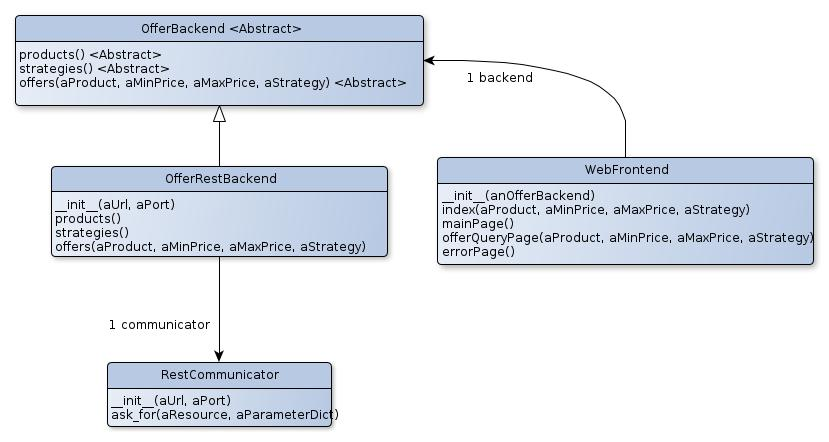
\includegraphics[scale=0.6]{graphics/frontend_class.jpg}
\caption{Frontend}
\end{figure}
\newpage

\subsection{REST Api}
Luego de que el \emph{Backend} haga su pedido a trav\'es de \emph{RestCommunicator} el mismo llegara a nuestra \emph{REST Api}. Para lograr esto utilizamos de nuevo a \emph{CherryPy} que nos provee un mensaje \emph{quickstart} para elegir una clase que hará el manejo de dichos pedidos. El siguiente diagrama ilustra dicha clase. El resto de las colaboraciones con estas clases ser\'an explicadas en detalle durante secciones posteriores.

\begin{figure}[H]
\centering
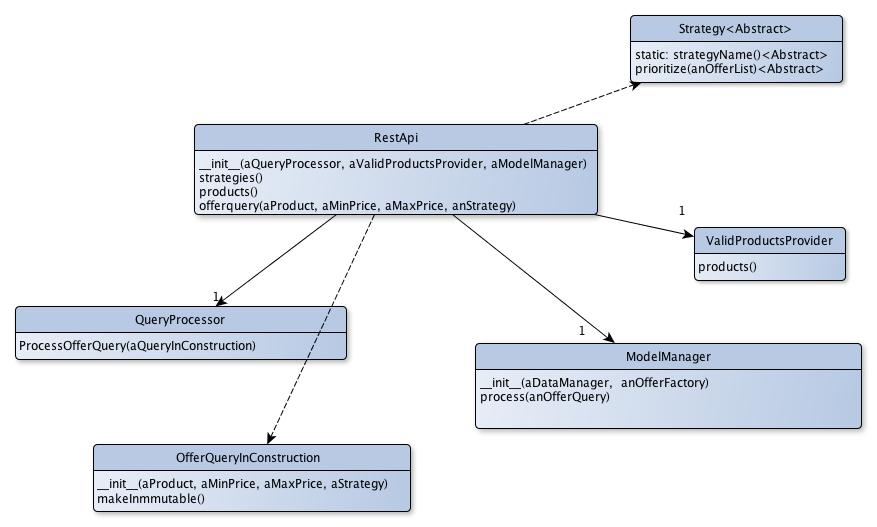
\includegraphics[scale=0.5]{graphics/rest_api_class.jpg}
\caption{RestApi class}
\end{figure}

El comportamiento m\'as interesante se encuentra en el mensaje \emph{offerquery}. El diagrama de secuencias debajo presenta el comportamiento global del \textbf{Backend}, iniciado por el mensaje \emph{offerquery} recibido por la \textbf{RestApi}, clase que se encarga de la comunicación con el exterior. Esta clase sabe traducir desde y hacia el lenguaje externo, en este caso el protocolo \textsf{Rest} y el lenguaje \textsf{Json}. La funcionalidad luego de la misma es recibir el mensaje en formato \emph{rest}, convertirlo en una \emph{query} de nuestro modelo llamando a un \textsf{QueryProcessor}, para así obtener una \textsf{OfferQuery}. Esta \textsf{OfferQuery} se le pasa al \textsf{ModelManager} que nos devolverá el resultado deseado y que \textsf{RestApi} se encargará de traducir al lenguaje utilizado en el exterior de la aplicación.
\begin{figure}[H]
\centering
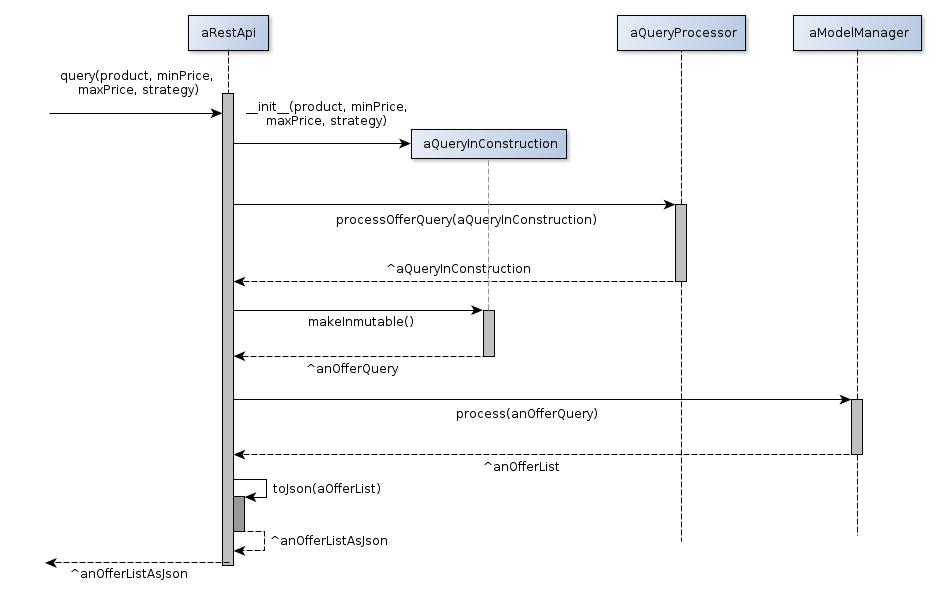
\includegraphics[scale=0.5]{graphics/service_sequence.jpg}
\caption{RestApi sequence}
\end{figure}

\subsection{QueryConstruction}
En esta secci\'on explicaremos con mas detalle el proceso y el diseño involucrados en la construccion de \emph{querys} que ocurre en los primeros mensajes del diagrama previo (\emph{RestApi sequence}). 

En este diagrama se destacan las clases de objetos que se encargan de, dada una \textbf{OfferQueryInConstruction} (Objeto que representa una consulta por ofertas sin procesar), construir el conjunto de restricciones a aplicar sobre las ofertas. Son los objetos de tipo \textbf{QueryProcessor} los encargados de construir los \textbf{Filter} y \textbf{Strategy} que determinan cuales serán los resultados finales de la consulta. En caso de que alguno de los párametros introducidos por el usuario no sean válidos, el \textbf{QueryProcessor} correspondiente informará de esta situación mediante una excepción. La clase \textbf{QueryProcessor} y sus subclases, siguen el patron de diseño \emph{Composite}.

Los objetos de tipo \textbf{ValidProductsProvider} llevan cuenta de cuales son los productos válidos. Un objeto de este tipo es utilizado por un \textbf{ProductQueryProcessor} para verificar que el producto ingresado por el usuario se encuentre en la lista de los productos soportados por el sistema.

\begin{figure}[H]
\centering
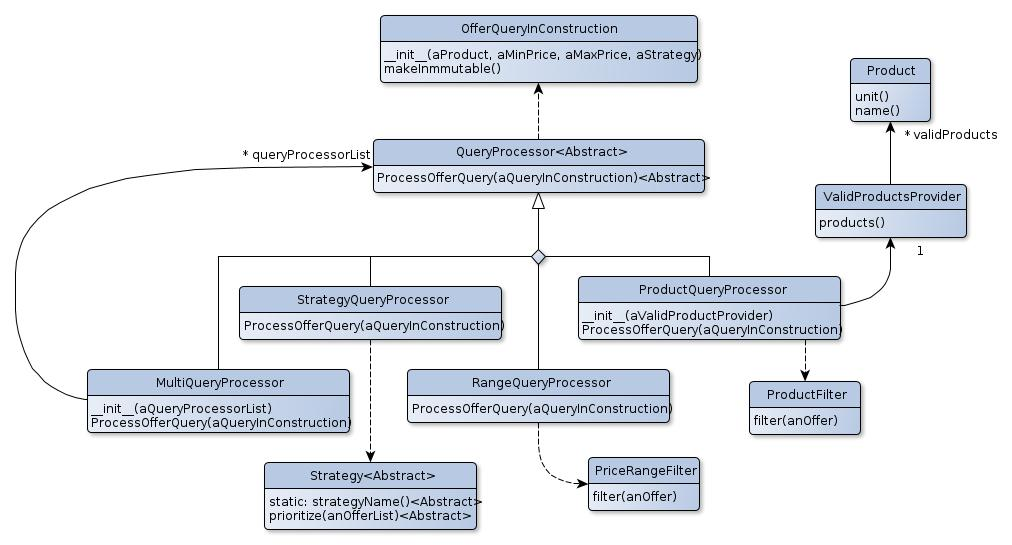
\includegraphics[scale=0.5]{graphics/queryProcessor_class.jpg}
\caption{Query Processor}
\end{figure}

Como fue mencionado anteriormente, un objeto de tipo \textbf{OfferQueryInConstruction} representa una query del usuario, la cual todavía no se terminó de procesar. Una vez que se terminaron de construir los filtros y estrategias correspondientes a la consulta del usuario, es necesario hacerla inmutable, obteniendo así un objeto con tipo \textbf{OfferQuery}. Los objetos de esta clase poseen únicamente un \textbf{Filter} y una \textbf{Strategy}.

Las \textbf{Strategy} representan distintas políticas para priorizar ofertas, por ejemplo, \emph{Mas baratas primero}. Los \textbf{Filter} representan condiciones booleanas que deben cumplir las ofertas para poder encontrarse en el conjunto de resultado. La clase \textbf{Filter} cumple con el patrón de diseño \emph{Composite}. La clase \textbf{MultiFilter} sigue el patrón \emph{TemplateMethod}, esta clase define un esqueleto para la función \emph{filter}, sin embargo, son las clases derivadas las que implementan los métodos \emph{reduceOp} y \emph{baseCase}.

\begin{figure}[H]
\centering
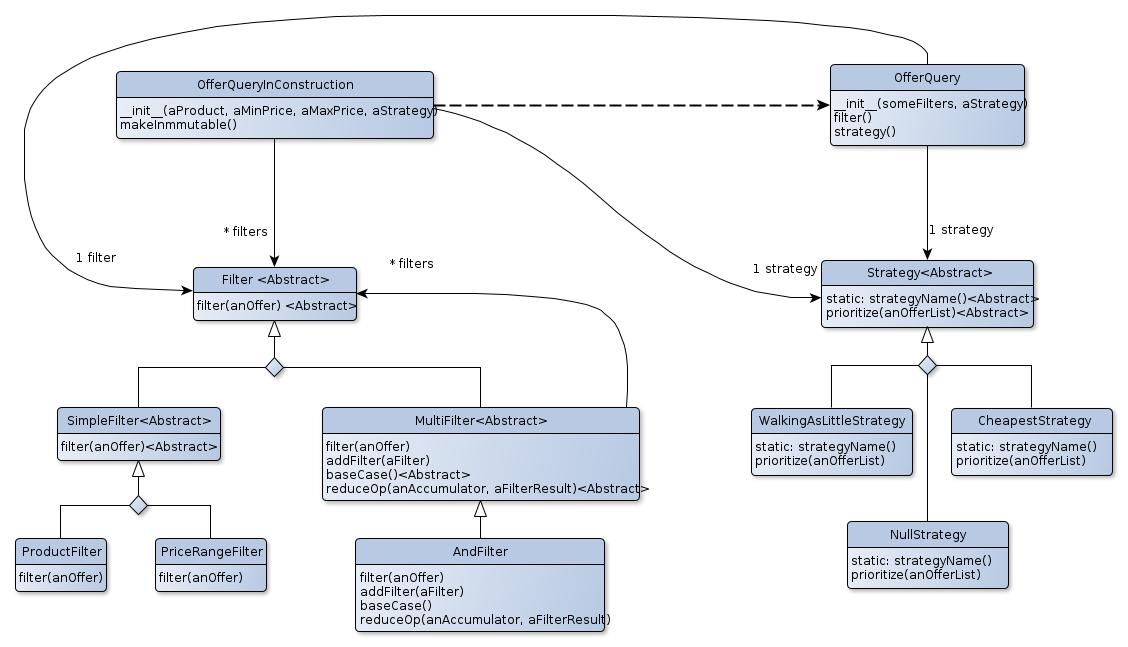
\includegraphics[width=\textwidth]{graphics/filter_class.jpg}
\caption{Filters and Strategies}
\end{figure}

\subsection{Filters}

En el siguiente diagrama se presenta el diagrama de secuencia para un \textbf{AndFilter}, que posee como colaborador a un \textbf{ProductFilter} y un \textbf{PriceRangeFilter}. Un \textbf{AndFilter} es un filtro que da su aprobación cuando todos los filtros contiene internamente también dan su aprobación. La interacción que se captura en este diagrama es la del mensaje \emph{filter} con \emph{anOffer} pasada como parámetro, a un \textbf{AndFilter}. El método asociado a este mensaje está implementado en \textbf{MultiFilter}. 

 Este método envia los mensajes \emph{baseCase} y \emph{reduceOp} a sí mismo. Los métodos asociados a estos mensajes están implementados en \textbf{AndFilter}. \emph{baseCase} es utilizado para inicializar un acumulador interno, mientras que \emph{reduceOp} se aplica a este acumulador y al resultado de aplicar cada filtro.
\begin{figure}[H]
\centering
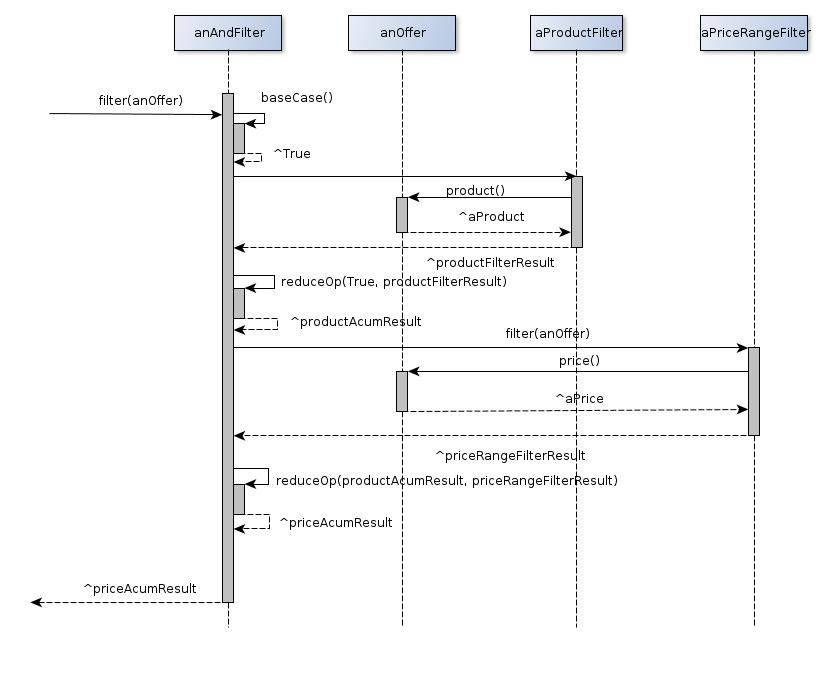
\includegraphics[scale=0.55]{graphics/andFilter_sequence.jpg}
\caption{andFilter}
\end{figure}
 
% Mostraremos a continuaci\'on un ejemplo de como es la interacci\'on que se produce cuando enviamos el mensaje \emph{filter(anOffer} a un filtro compuesto por otros dos, uno por productos y el siguiente por precios. Esta interacci\'on sera referenciada despu\'es al momento de filtrar una oferta por los filtros de una \emph{query}
% 
\newpage
\subsection{OfferQueryProcessing}
El siguiente diagrama gira entorno a la clase \textbf{ModelManager}, cuya responsabilidad es procesar una \emph{query} contra las ofertas que el sistema encuentra en \emph{Twitter}. Su nombre nace de su interacción con sus colaboradores internos (\textbf{DataManager}, \textbf{OfferFactory}) y parámetros (\textbf{OfferQuery}). Para realizar el procesamiento de una \emph{query} el mismo debe ir interactuando uno a uno con los mismos. Dicha interacción resulta a nivel gr\'afico en una forma de estrella.

El primer eje de cambio que tuvimos en consideración y se ve reflejado en el diagrama es la posibilidad de tener más de una fuente de datos adem\'as de la REST api de \emph{Twitter}. Este eje se logra facilmente agregando otro \textbf{DataSource} concreto a la instancia de  DataManager con el m\'ensaje \emph{addConnector}.

El siguiente eje de cambio est\'a en el uso de la interfaz \emph{iterable} por \textbf{OfferFactory}, \textbf{OfferFactory} la utiliza para iterar los datos que provee \textbf{DataManager} y esto genera un desacoplamiento ya que lo unico que \textbf{OfferFactory} necesita es un tipo de almacenamiento de datos que provea una manera de iterarlos mediante el mensaje \emph{next()}. Por ejemplo, en siguientes versiones del sistema podría utilizarse algun mecanismo de persistencia que ayude a eliminar el costo de hacer el request a nuestros conectores cada vez y la clase \textbf{OfferFactory} no deber\'ia modificarse. 

\begin{figure}[H]
\centering
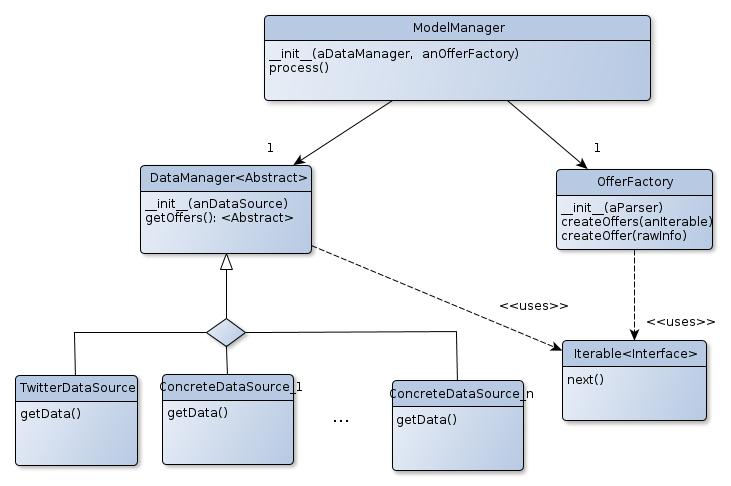
\includegraphics[scale=0.50]{graphics/model_manager_iterable_class.jpg}
\caption{Model Manager Class}
\end{figure}

La interacci\'on primordial de \textbf{ModelManager} esta en el mensaje \emph{process(anOfferQuery)} que es llamado por \textbf{RestApi} luego de el armado de la \emph{anOfferQuery} visto en la secci\'on previa. Vemos entonces como esta compuesta esta interacci\'on en el siguiente diagrama. 

\begin{figure}[H]
\centering
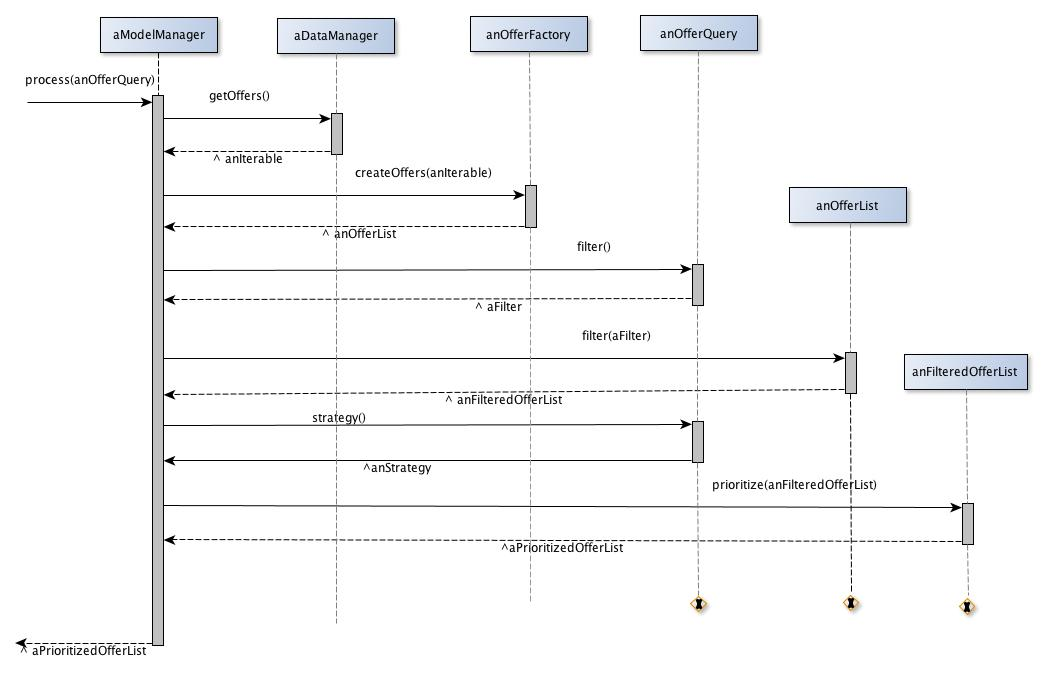
\includegraphics[scale=0.50]{graphics/modelManager_sequence.jpg}
\caption{Model Manager Sequence}
\end{figure}

En esta secuencia se vislumbra lo que viene en la pr\'oxima secci\'on vinculada al armado de \emph{ofertas} desde los datos obtenidos desde \emph{Twitter} con el mensaje \emph{getOffers()}.Luego de obtener un iterador de los datos se delega en \textbf{OfferFactory} la responsabilidad de traducci\'on, parseo y validaci\'on de los datos iterables hasta devolver una lista de ofertas.

\newpage
\subsection{Offer Building with OfferFactory}

Para pasar de los Tweets (u otro medio, ya que en este punto es transparente el origen de la información) a ofertas entendibles en nuestro sistema. Implementamos un \textbf{OfferFactory} el cual es capaz de transformar una lista de tweets (validos o no) en una lista de ofertas válidas.\\

Para esto el OfferFactory es inicializado con un \textbf{ParserChain} que se encarga de intentar parsear la información de los twists devolviendo como resultado un \textbf{OfferBuilder} o la excepción  \textbf{ParserError} en caso de no ser posible para el parser extraer la información para rellenar el OfferBuilder.\\

El ParserChain es Inicializado con una lista de \textbf{SpecificParser}, los cuales son llamados en el orden en el que vienen en la lista, tratando de extraer la información que necesitan y volcándola dentro del OfferBuilder que se está rellenado.\\

Este diseño nos da una gran flexibilidad para los cambios futuros, tanto en agregar nuevas formas de extraer datos, como también alterar la forma en la que se extraen los dados ahora sin modificar otras.\\

Como por ejemplo sería muy fácil agregar el validador ortográfico para poder detectar productos mal escritos sin necesidad de alterar ninguna otra parte (en el diseño se muestra una clase tentativa que le agrega a \textbf{ProductParser} la posibilidad de chequear esto).\\

Lo mismo se aplica con la posibilidad de agregar validaciones a la \textbf{Location} la cual por el momento solo consiste en un string que no tiene ningún tipo de chequeo sobre su validez.\\ 



\begin{figure}[H]
\centering
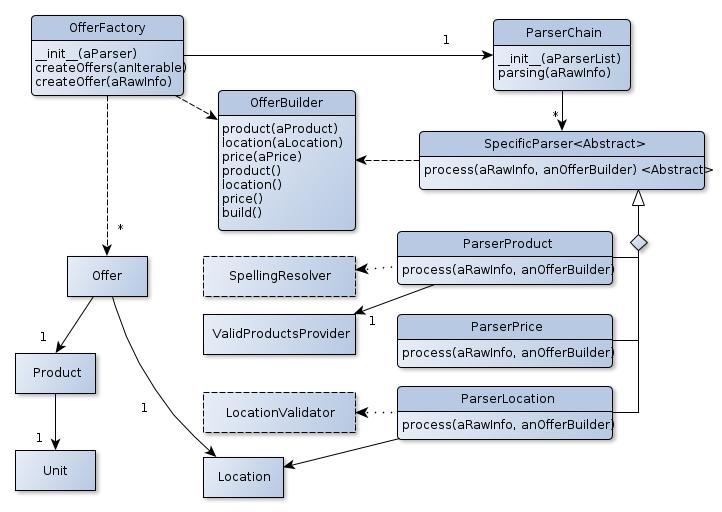
\includegraphics[scale=0.65]{graphics/parser_class.jpg}
\caption{Offer Factory}
\end{figure}

 
\begin{landscape}

En este diagrama se muestra el envío del mensaje \emph{createOffers} a un \textbf{OfferFactory} pasándole como parámetro un objeto Iterable, este almacena un conjuntos de objetos del tipo \textbf{RawInfo} los cuales pueden ser pedidos uno tras otro utilizando el mensaje \emph{next}. \\

En este caso particular el objeto Iterable va a tener dos elementos en su interior, de los cuales el primero es un dato válido ya que el objeto RawInfo contiene un text parseable por el sistema(ej:"Leche a 5 p el lt en varela al 20 \#precioJusto"), mientas que el segundo contiene información no parseable(ej:"los mejores productos \#precioJusto").
\begin{figure}[H]
\centering
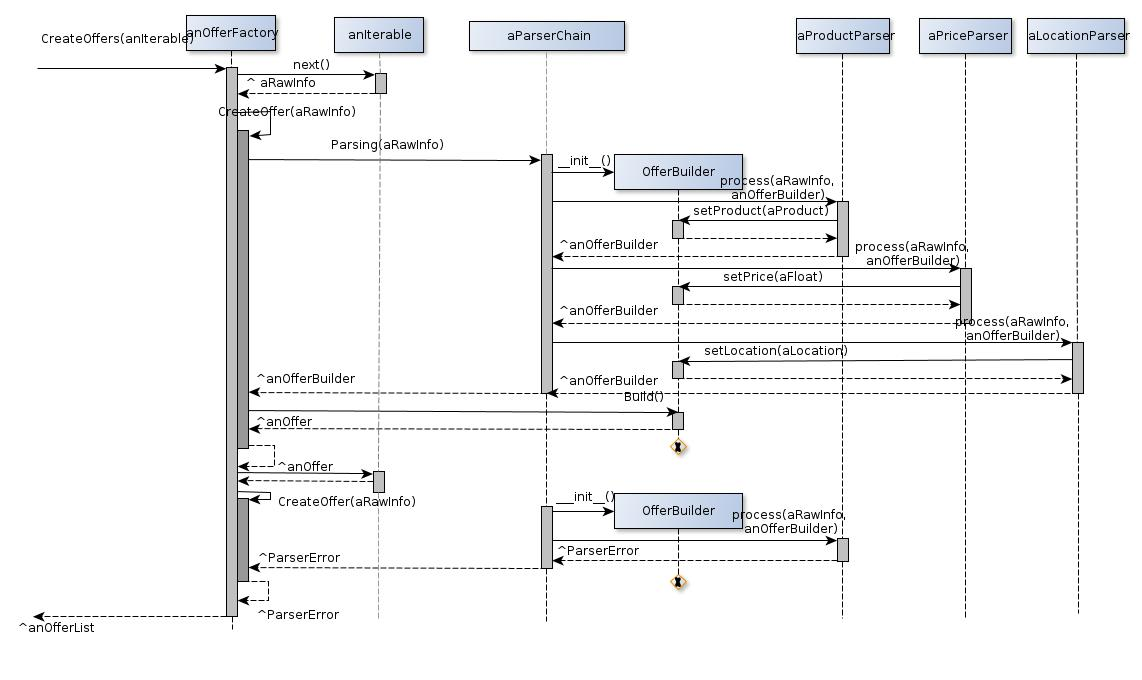
\includegraphics[scale=0.55]{graphics/OfferFactory_sequence.jpg}
\caption{Offer Factory}
\end{figure}

\end{landscape}


%\newpage
%\subsection{Propuesta de extension sobre Obtenci\'ion de datos}
%Durante el transcurso del trabajo vimos que existen varias formas de conseguir informacion desde \emph{Twitter} asi como varias maneras de almacenarla. Por ejemplo uno puede obtener informaci\'on desde la api \emph{REST} o por la api de \emph{Streaming} y esta misma informaci\'on puede ser persistida en un archivo de texto plano, en memoria o en alguna base de datos. En el siguiente diagrama ilustramos una propuesta para diseniar un sistema capaz de soportar estas formas de obtenci\'on de datos y de persistencia. El mismo no cumple con condiciones deseables de un disenio orientado a objetos y por eso mismo el codigo de nuestro trabajo no se corresponde con esta propuesta. Pero a\'un as\'i nos parece interesante exponerla dentro de este informe.
%
%
%
%\begin{figure}[H]
%\centering
%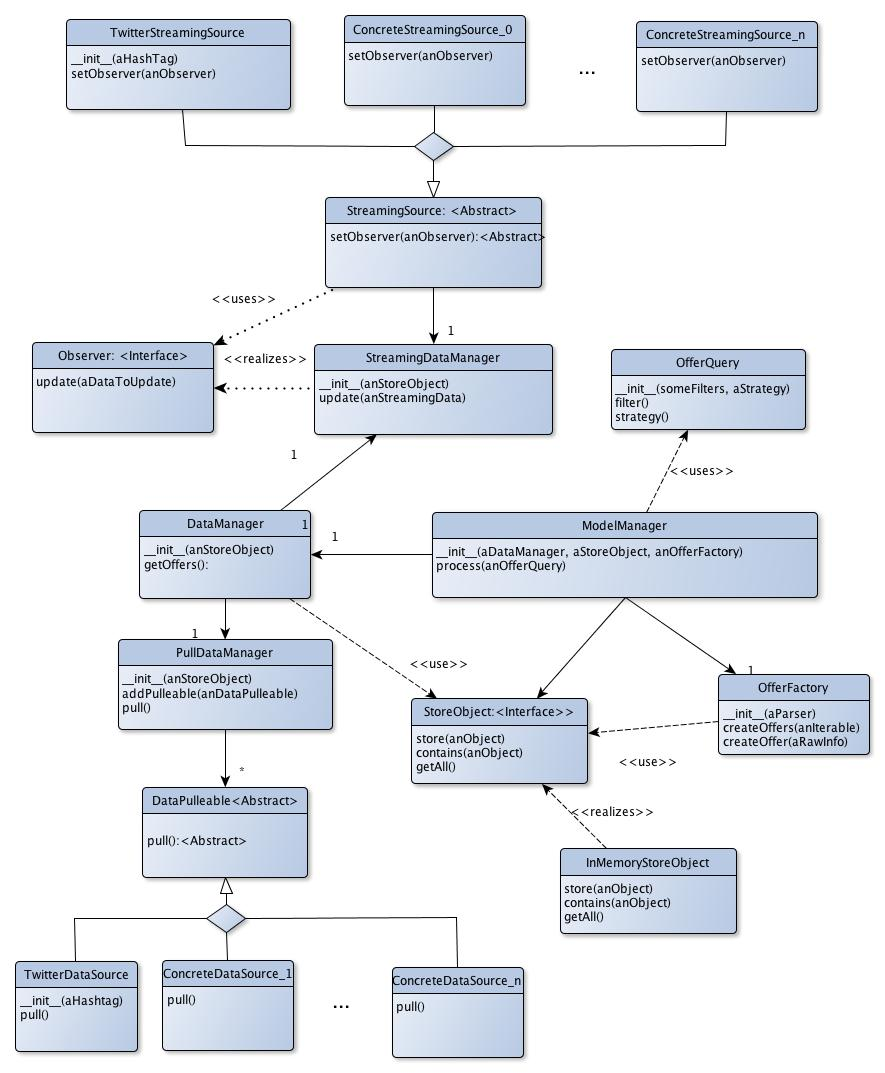
\includegraphics[scale=0.6]{graphics/model_manager_storeObject_class.jpg}
%\caption{Model Manager StoreObject}
%\end{figure}


\section{Primera Iteración}

En un esquema de desarrollo iterativo incremental, el producto final se construye en iteraciones. En cada iteración se establecen ciertos objetivos, que apuntan a agregar una nueva funcionaliad al producto. Para el momento de este informe, se desarrolló solo la primera iteración. En la misma, el objetivo definido fue tener una primera versión de la aplicación con una funcionalidad limitada, pero completa frente al espíritu del proyecto. El resultado de una iteración se denomina \emph{product increment} y deberá permitir buscar las ofertas de un producto en \emph{twitter}, filtrarlos con algún criterio y priorizalos mediante alguna estrategia.

A continuación explicamos cómo resulto el desarrollo de la primera iteración.

\subsection{Desarrollo}

En el ámbito del trabajo que se está realizando, es importante remarcar el hecho que el desarrollo iterativo incremental de la aplicación fue en el marco de un trabajo práctico cuyos objetivos exceden (e incluso son conflictivos con) los objetivos normales de una iteración. Es así que el trabajo se dividió en dos aristas: la de \emph{diseño orientado a objetos} y la de \emph{desarrollo del increment}. 

Lo primero que se hizo fue definir los requerimientos y el alcance de la aplicación al generar el \emph{Product Backlog}, cuyas historias detallarían estas decisiones. Luego surgió la necesidad de enfocarnos completamente en el diseño de la aplicación, lo que conformaba un punto muy importante del trabajo práctico. Esta sección de trabajo entra en conflicto con la metodología de desarrollo ya que en la misma la visibilidad completa del diseño no solo no es importante sino que debe postergarse para extenderse y corregirse contínuamente con las iteraciones. A razón de este trabajo inicial de diseño el desarrollo quedó en segundo plano hasta la segunda mitad del \emph{sprint}, como puede verse en el \textbf{burndown chart}.

\begin{figure}[H]
\centering
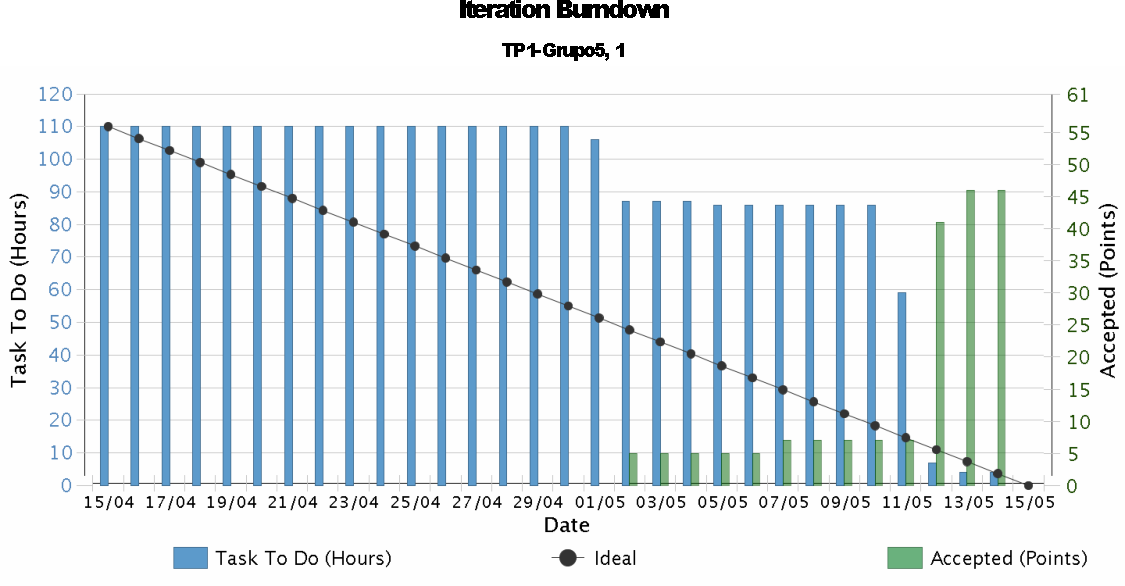
\includegraphics[width=\textwidth]{graphics/iteration_burndown.pdf}
\caption{\textbf{Burndown chart:} progreso de terminación de tareas en el \emph{sprint}.}
\end{figure}

Una vez contentos con el porcentaje de diseño realizado para los fines del trabajo práctico, el desarrollo de código adquirió prioridad. Considerando que los integrantes del equipo, teniendo otras responsabilidades, no podían dedicarse diariamente al proyecto, puede observarse en el gráfico que los días de trabajo están espaciados. Las actividades de finalización de tarea fueron bastante postergadas, por lo que la cantidad de historias aceptadas creció abrúptamente en los últimos días.

\subsection{Logros}

El primer \emph{product increment} se enfocó en lograr una primera prueba de un sistema funcionando completamente. Su desarrollo se orientó a que hubiera algo para presentar al \emph{Product Owner} y al usuario final, así como para que fuera fácilmente expansible a los ejes de cambio definidos. Entre las funcionalidades básicas logradas se encuentran:

\begin{itemize}
  \item Un frontend web que permite simple usabilidad para el usuario.
  \item Consulta a \emph{twitter} de tweets con hashtag \textbf{\#PrecioJusto} para obtener precios de productos.
  \item Interpretación de los \emph{tweets} para obtener la información.
  \item Priorización de los menores precios encontrados para un producto.
  \item Filtrado de los precios acorde a un mínimo y máximo.
\end{itemize}

\subsection{Revisión}

Al finalizar el \emph{sprint} realizamos una revisón sobre cómo trabajó el equipo y qué mejoras podrían hacerse. Llegamos a las siguientes conclusiones. 

\begin{itemize}
  \item \textbf{Poca comunicación con el PO:} a lo largo del \emph{sprint}, la falta de comunicación con el \textbf{Product Owner} originó muchas sorpresas en cuanto a requerimientos y expectativas tanto del desarrollo del \emph{increment} como del trabajo práctico. En futuras iteraciones es recomendable reunirse con el \textbf{Product Owner} con mayor frecuencia.
  \item \textbf{Seguimiento espaciado del proyecto:} a causa de otras responsabilidades y distracciones, las horas dedicadas al desarrollo estuvieron espaciadas y la mayor parte del trabajo se concentró en unos pocos días. En el futuro es recomendable una mayor frecuencia de trabajo de forma que los desvíos y las dudas puedan resolverse con mayor velocidad.
  \item \textbf{Poco asado:} evidentemente el trabajo del equipo se vio afectado por la falta de asado en las reuniones, que bajó la moral y denigró el espíritu de trabajo. En las próximas iteraciones la bondiola y vacío serán protagonistas.
  \item \textbf{Disparidad en la formación de los integrantes:} a causa de las distintas experiencias y líneas de trabajo de cada uno de los integrantes, nos encontramos con diferencias en la experiencia con las herramientas y variedad de forma de pensar las problemáticas. En el futuro será importante tener en cuenta que es necesario dedicarle más atención a cómo comunicamos las ideas dentro del equipo, así como equiparar mejor el conocimiento de las tecnologías.
\end{itemize}



\end{document}
